Предполагается, что базовый алгоритм специализации должен быть хуже по
скорости и, в некоторых случаях, по качеству специализации.
Данная работа не затрагивает способы повышения эффективности процесса
суперкомпиляции, однако демонстрирует некоторые продвижения в эту сторону
из-за чисто прагматических соображений. Основное внимание уделяется
подходам к суперкомпиляции и их влиянию на суперкомпиляционные эффекты.

\subsubsection{Стратегии свёртки}
% \textbf{Поиск узлов для переименования среди всех вычисленных поддеревьев}

В базовом алгоритме суперкомпиляции поиск узлов на которые происходят переименования
происходит среди родителей. Это напрямую соотносится с понятием символьных
вычислений: по достижении узла, который является переименованием уже встреченного,
вычисление переходит на родительский узел. Однако довольно часто встречается
такая ситуация,
что в разных поддеревьях дерева процессов встречаются одинаковые конфигурации,
поддеревья которых оказываются полностью идентичными. В таком случае, кажется
очевидной и несложной оптимизация, при которой запоминаются вычисленные
поддеревья и в случае, когда встречается схожая конфигурация,
поддерево не вычисляется заново, а добавляется ссылка на него.

% \todo{Вопрос на засыпку меня же: может ли быть такое, что конфигурации
% являются вариантами друг друга, но накопленные подстановки приведут к появлению
% различных поддеревьев?}\\

%%%%%%%%%%%%%%%%%%%%%%%%%%%%%%%%%%%%%%%%%%%%%%%%%%%%%%%%%%%%%%%%%%%%%%%%%%%%%%
%%%%%%%%%%%%%%%%%%%%%%%%%%%%%%%%%%%%%%%%%%%%%%%%%%%%%%%%%%%%%%%%%%%%%%%%%%%%%%
%%%%%%%%%%%%%%%%%%%%%%%%%%%%%%%%%%%%%%%%%%%%%%%%%%%%%%%%%%%%%%%%%%%%%%%%%%%%%%
%%%%%%%%%%%%%%%%%%%%%%%%%%%%%%%%%%%%%%%%%%%%%%%%%%%%%%%%%%%%%%%%%%%%%%%%%%%%%%

\subsubsection{Стратегии развёртки}
% \textbf{Стратегии развёртывания реляционных вызовов}\\

Как уже говорилось, разные стратегии развёртывания реляционных вызовов могут
привести к разным эффектам специализации. К примеру, полная стратегия развёртывания,
которая была принята за базовую, может приводить к дефорестации, описанной ранее.

Основной недостаток базового подхода в том, что для получения всех возможных
состояний он производит декартово произведение нормализованных состояний тел
вызовов в конъюнкциях, что приводит к сильному разрастанию и дерева процессов и,
как следствие, сильно требователен к вычислительным ресурсам и приводит
к большой ветвистости программ. Последнее оказывает негативный эффект на процесс
вычисления и может ухудшить производительность.
Вследствие чего реализация новых стратегий развёртывания производится
в исследовательских и прикладных целях.

Для лёгкой подмены стратегий суперкомпиляции был разработан специальный интерфейс \lstinline{Unfoldable}
(рисунок~\ref{fig:unfoldable}).
\begin{figure}[h!]
\begin{lstlisting}
class Unfoldable a where
   initialize :: Conf $\rarrow$ a
   get        :: a $\rarrow$ Conf
   unfold     :: a $\rarrow$ Env $\rarrow$ List (Env, a)
\end{lstlisting}
\caption{Интерфейс для различных стратегий развёртывания.}
\label{fig:unfoldable}
\end{figure}

Предоставляемые интерфейсом функции используются в алгоритме суперкомпиляции следующим образом:
\begin{itemize}
\item \lstinline{initialize} оборачивает конфигурацию в структуру, в которой может содержаться
      вспомогательная информация для процесса развёртывания;
\item \lstinline{get} позволяет получить конфигурацию для её применения к операциям, не зависящим
      от стратегий;
\item \lstinline{unfold} непосредственно проводит шаг вычисления на основе текущей конфигурации
      и её окружения, порождая новые конфигурации с соответствующими им состояниями.
\end{itemize}

В работе рассмотрен и реализован ряд стратегий, описанных ниже.

\begin{itemize}
\item {\bf Модифицированная полная стратегия развёртки}, при которой сначала из цели
      раскрываются все нерекурсивные вызовы.
      Нерекурсивность определяется
      лишь тем, содержит ли определение реляционный вызов самого себя. Более сложный
      анализ структуры функций не мог бы быть использован в силу того, что тогда
      было бы необходимо реализовать класс алгоритмов анализа, что совершенно отдельная задача.

\item {\bf Стратегия развёртывания самого первого элемента}, при которой ожидается,
      что конфигурации не будут часто разбиваться на подконъюнкции, что может
      привести к оптимизационным эффектам, схожим с полным развёртыванием.

\item {\bf Последовательная стратегия развёртывания}, при которой отслеживается,
      какой вызов был раскрыт на предыдущем шаге, чтобы на текущем
      раскрыть следующий за ним. Ожидается, что в этой стратегии
      при суперкомпиляции будут учтены, так или иначе, все или большинство конъюнтов
      конфигурации.

\item {\bf Нерекурсивная стратегия развёртывания}, являющаяся модификацией
      последовательной стратегии, при которой в первую очередь
      раскрывается нерекурсивный вызов в конфигурации.

      Ожидается, что при нерекурсивной стратегии развёртывания из конфигураций
      будут как можно быстрее появляться выражения, которые могут быть сокращены
      или вовсе удалены из-за унификации (к примеру, отношения, кодирующие
      таблицы истинности, такие как \rel{and}) или привести к скорой свёрткке.

\item {\bf Рекурсивная стратегия развёртывания}, являющаяся модификацией
      последовательной стратегии,  при которой в первую очередь
      раскрывается рекурсивный вызов в конфигурации. Ожидается, что это
      может привести к скорому обобщению.

\item {\bf Стратегия развёртывания вызовов с минимальным количеством ветвлений},
      при которой на каждом шаге вычисления будет появляться минимально возможное количество
      конфигураций, что приведёт к минимальной ветвистости дерева.

\item {\bf Стратегия развёртывания вызовов с максимальным количеством ветвлений},
      при которой на каждом шаге вычисления будет появляться максимально возможное количество
      конфигураций, что, с одной стороны, увеличит количество возможных состояний, но
      потенциально может привести к скорому сворачиванию или обобщению.

\end{itemize}

% \subparagraph{Смешанная стратегия развёртывания}
% \todo{Ещё нужно бы проработать}

%%%%%%%%%%%%%%%%%%%%%%%%%%%%%%%%%%%%%%%%%%%%%%%%%%%%%%%%%%%%%%%%%%%%%%%%%%%%%%
%%%%%%%%%%%%%%%%%%%%%%%%%%%%%%%%%%%%%%%%%%%%%%%%%%%%%%%%%%%%%%%%%%%%%%%%%%%%%%
%%%%%%%%%%%%%%%%%%%%%%%%%%%%%%%%%%%%%%%%%%%%%%%%%%%%%%%%%%%%%%%%%%%%%%%%%%%%%%
%%%%%%%%%%%%%%%%%%%%%%%%%%%%%%%%%%%%%%%%%%%%%%%%%%%%%%%%%%%%%%%%%%%%%%%%%%%%%%
\subsubsection{Стратегии обобщения}

Для модификации стратегии обобщения были рассмотрены два подхода.

%\textbf{Обобщение на все вычисленные узлы, не только на родительские}
% \todo{Понять, почему это не противоречит методам суперкомпиляции}

Во-первых, увеличение множества рассматриваемых конфигураций, на которые
производится обобщение, до всех уже рассмотренных конфигураций.

Покажем, что допустимо использовать обобщение на все вершины.
Для этого рассмотрим конфигурацию $C_w$ и некоторую конфигурацию $C_p$ из множества
конфигураций для обобщения, расширенное всеми уже обработанными конфигурациями.
При обобщении $C_p$ и $C_w$ породится множество дочерних конфигураций, % $\{ C_w^i \}$,
каждая из которых будет более общим подконъюнтом $C_w$ и, в силу своей
обобщённости, будет содержать меньше информации, чем исходная конфигурация,
однако не будет ей противоречить. В итоге, обобщение на все обработанные
вершины влияет только на то, каким образом разбивается рассматриваемая
конфигурация, что может привести к скорой свёртке, и как много информации о
переменных теряется. 

%Если $C_p$ является предком $C_w$, тогда ничего не нарушается.
%Иначе, 
% В ином случае, рассмотрим более внимательно эти конфигурации.
% По определению, $C_p \embed^+ C_w$ и 

Обобщение на вычисленные узлы приводит к тому, что деревья конфигураций
быстрее сходятся, однако остаётся под вопросом, ухудшает ли этот подход
качество специализации. 

Во-вторых, допустимо ввести модификацию, которая запрещает прозводить операцию
обобщения, если родительская конфигурация была получена с помощью обобщения.
Такая эвристика может привести к том, что программы будут чаще развёртываться,
однако в купе с другими модификациями может привести к интересным результатам.

% \textbf{Реализация обобщения вверх}

В-третьих, в суперкомпиляции, в отличие от методов частичной дедукции, для обобщения дополнительно может использоваться
техника обобщения вверх, при которой происходит не подвешивание обобщённой конфигурации
в качестве потомка конфигурации, которая обобщалась, но замена самого родителя на
новую конфигурацию~\cite{scPos}. Старое же поддерево родителя уничтожается.

Для определения необходимости обобщать вверх введём предикат $e_1 \genup e_2$,
который определяет, что $e_1 \strictinst e_2$ и $e_2 \not\strictinst e_1$.
Такое ограничение необходимо из-за того, что суперкомпилятор оперирует
конъюнкциями выражений и делает операции разделения и обобщения вниз
за один шаг с конъюнкциями возможно разной длины, однако для обобщения
вверх необходимо удостовериться, что замена родительского дерева, во-первых,
не добавит конфигураций, которых там не может быть, во-вторых, предоставит
только более общую информацию.

\begin{figure}[h!]
\begin{lstlisting}
  else if $\exists$ parent: parent $\genup$ configuration
  then
     node $\larrow$ generalize(configuration, parent)
     addUp(env, tree, parent, node)
\end{lstlisting}
\caption{Расширение алгоритма суперкомпиляции.}
\label{fig:scalgogenExtended}
\end{figure}

Наличие операции обобщения вверх предполагает, что необходимо умение передвигаться по дереву вверх и изменять его.
Реализация в Haskell этой идеи --- задача крайне нетривиальная. Возможно представлять
деревья в мутабельных массивах, однако при обобщении необходимо удалять целые поддеревья,
что при таком подходе сложная операция.

Классическим способом решения этой проблемы являются \emph{зипперы}~\origin{zipper}~\cite{zipper},
на основе которых, к примеру, создан система для суперкомпиляции,
представленная в работе ~\cite{optimus}.

Идиома зипперов предлагает рассматривать структуру данных как пару из элемента,
на котором установлен фокус, и контекста, который представляется как структура данных
с ``дыркой'', в котором сфокусированный элемент должен находиться.
К примеру, зиппер для списка \lstinline{[1, 2, 3, 4, 5]} при фокусе на 3 представляется
таким образом: \lstinline{(3, ([2, 1], [4, 5]))}.
Тогда перефокусировка вправо или влево на один элемент происходит за константное время,
как и замена элемента, для которой достаточно заменить первую компоненту пары.
В то время как, в силу того, что операция взятия элемента в связном списке по индексу
происходит за линейное время от длины списка, взятие элемента слева от 3 также
будет происходить за линейное время, как и, соответственно, модификация списка.
Для деревьев с произвольным количеством детей зиппер может выглядеть
как пара из текущего узла и списка родителей, отсортированного в порядке
близости к узлу (рисунок~\ref{fig:zipper}).

\begin{figure}[h!]
\begin{lstlisting}[mathescape,language=Haskell,extendedchars=\true,frame=single,basicstyle=\ttfamily]
data Parent = Parent { children :: ListZipper Node }
type TreeZipper = (Node, List Parent)
\end{lstlisting}
\caption{Пример структуры зиппера для деревьев}
\label{fig:zipper}
\end{figure}

Родительский (структура \lstinline{Parent}) cписок детей представлен в виде зиппера (поле \lstinline{children})
для списка, в котором происходит фокус: у непосредственного родителя --- на элемент в фокусе, а у остальных
родителей --- на предыдущего в порядке сортировки.
Тогда передвижение вверх до первого подходящего узла происходит путём
заполнения дыры при переходе на родителя, а передвижение в левого брата ---
простой сдвиг в зиппере списка \lstinline{children}.

При представлении дерева процессов в идиоме зипперов основа алгоритма
суперкомпиляции принимает форму описания действий при смене состояния зиппера.
Дерево всё ещё строится в глубину и происходит это следующим образом:
если мы в узле, порождающем другие узлы (то есть \lstinline{Unfolding}
или \lstinline{Abstraction}), то порождённые узлы добавляются в дерево
с пометкой о том, что они не достроены, а алгоритм спускается в первого
ребёнка. Когда же алгоритм приходит в листовой узел, то ему нужно подняться
до родителя, у которого существует помеченный потомок, и спуститься в этого
потомка. Алгоритм завершается, когда не осталось помеченных детей.

Обобщение вверх приводит к тому, что происходит замена целого поддерева процессов
предка, на которого обобщается конфигурация. Иногда это может приводить к потере
связи между аргументами, из-за чего исчезает потенциал для возможных
положительных эффектов, к примеру, протягивания констант.

К примеру, на рисунке~\ref{fig:genup} представлено дерево процессов, при котором происходит обобщение вверх.

\begin{figure}[h!]
\center
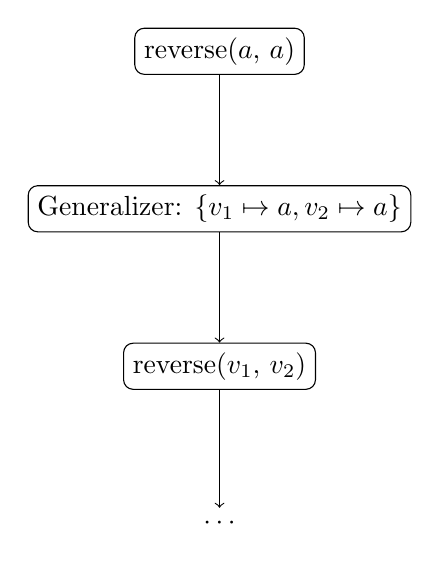
\begin{tikzpicture}[->,node distance=2cm, sibling distance=5cm]
                                                       
\tikzstyle{conf}=[rectangle,draw, rounded corners=.8ex]
\node[conf] (root) {\rel{reverse}($a$, $a$)} ;
\node[conf] (gen) [below of = root] {Generalizer: $\{ v_1 \mapsto a, v_2 \mapsto a \}$};
\node[conf] (node) [below of = gen] {\rel{reverse}($v_1$, $v_2$)};
\node (rest)[below of = node] {$\cdots$};
\path (root) edge (gen)
      (gen) edge (node)
      (node) edge (rest);
\end{tikzpicture}
\caption{Демонстрация потери информации при обобщении вверх.}
\label{fig:genup}
\end{figure}

C одной стороны, теряется потенциал для генерации более оптимальной для цели \rel{reverse}($a$, $a$)
программы, но c другой стороны рассмотрим следующие соображения.

В данном примере процесс прогонки происходил следующим образом: некоторое время строился
граф для конфигурации \rel{reverse}($a$, $a$), затем вывелась конфигурация \rel{reverse}($a$, $b$).
Если бы обобщения вверх не происходило бы, то поиск ответов в результирующей программе
малое время провёл бы в поддереве, оптимизированном под \rel{reverse}($a$, $a$), а остальное --- в обобщённом
\rel{reverse}($a$, $b$).

В общем случае это может происходить не только с корнем дерева, но и в каких-то его поддеревьях.
Однако запрет на обобщение вверх в поддеревьях может сгенерировать слишком много частных случаев
и привести к более неэффективным программам.

Из того, что, во-первых, есть потенциал оптимизации при сохранении информации в корне дерева и,
во-вторых, необходимо сдерживать разрастание дерева конфигураций,
допускается рассмотрение алгоритма с обобщением вверх с запретом на обобщение к корню дерева.

%%%%%%%%%%%%%%%%%%%%%%%%%%%%%%%%%%%%%%%%%%%%%%%%%%%%%%%%%%%%%%%%%%%%%%%%%%%%%%
%%%%%%%%%%%%%%%%%%%%%%%%%%%%%%%%%%%%%%%%%%%%%%%%%%%%%%%%%%%%%%%%%%%%%%%%%%%%%%
%%%%%%%%%%%%%%%%%%%%%%%%%%%%%%%%%%%%%%%%%%%%%%%%%%%%%%%%%%%%%%%%%%%%%%%%%%%%%%
%%%%%%%%%%%%%%%%%%%%%%%%%%%%%%%%%%%%%%%%%%%%%%%%%%%%%%%%%%%%%%%%%%%%%%%%%%%%%%

\subsubsection{Расширение \ukanren оператором неэквивалентности}

Множество операций в оригинальном \ukanren покрывает все нужды реляционного программирования,
однако на ряде программ оно вычислительно допускает пути исполнения, которые не приводят
к успеху, однако сообщить об этом не представляется возможным.

К примеру, на рисунке~\ref{fig:lookup} изображена операция поиска значения по ключу
в списке пар ключ-значения \rel{lookup}.

\begin{figure}[h!]
\begin{lstlisting}
$\text{lookup}^o$ K L R =
   (K', V) :: L' $\equiv$ L $\land$
   (K' $\equiv$ K $\land$ V $\equiv$ R $\lor$ $\text{lookup}^o$ K L' R)
\end{lstlisting}
\caption{Отношения поиска значения по ключу.}
\label{fig:lookup}
\end{figure}

В соответствии с программой список \lstinline{L} должен иметь в голове пару из ключа и значения \lstinline{(K', V)}
и либо  этот ключ \lstinline{K'} унифицируется с искомым ключом \lstinline{K} и
значение \lstinline{V} --- с результатом \lstinline{R},
либо поиск происходит в хвосте списка \lstinline{L'}. Проблема этой программы в том,
что если унификация \lstinline{(K',V)::L' $\equiv$ L} прошла успешно и был
найден результат, то поиск всё равно продёт во вторую ветку с рекурсивным вызовом и будет
искать значение дальше, хотя по прагматике поиска ключа в списке должен вернуться лишь одно значение.
Более того, суперкомпилятору тоже придётся учитывать и, возможно, проводить вычисления,
которые не принесут никакой пользы.

В miniKanren существует операция неэквивалентности $t_1 \not\equiv t_1$, вводящая
ограничение неэквивалентности \origin{disequality contraints}\cite{mkConstr}.
Операция неэквивалентности определяет, что два терма $t_1$ и $t_2$ никогда не должны быть равны,
накладывая ограничения на возможные значения свободных переменных терма.

Расширение синтаксиса \ukanren представлено на рисунке~\ref{fig:syntaxExt}.

\begin{figure}[h!]
\centering
\[\begin{array}{ccll}
\mathcal{G}   & = & \hspace{1cm} \dots & \\
              &   & \hspace{1cm} \mathcal{T_X}\not\equiv\mathcal{T_X} \hspace{2cm} &\mbox{неэквивалентность} \\
\end{array}\]
\caption{Расширение синтаксиса \ukanren относительно указанного на рисунке~\ref{fig:syntax}.}
\label{fig:syntaxExt}
\end{figure}

Исправленная версия отношения \rel{lookup} представлена на рисунке~\ref{fig:lookupExt}.

\begin{figure}[h!]
\begin{lstlisting}
$\text{lookup}^o$ K L R =
   (K', V) :: L' $\equiv$ L $\land$
   (K' $\equiv$ K $\land$ V $\equiv$ R $\lor$
    K' $\not\equiv$ K $\land$ $\text{lookup}^o$ K L' R)
\end{lstlisting}
\caption{Исправленное отношение поиска значения по ключу.}
\label{fig:lookupExt}
\end{figure}

В такой реализации две по сути исключающие друг друга ветви исполнения будут исключать друг друга
и при вычислении запросов, и при суперкомпиляции.

Для реализации ограничения неэквивалентности вводится новая сущность под названием
``хранилище ограничений'' $\Omega$ \origin{constraints store}, которое используется для проверки
нарушений неэквивалентности. Окружение расширяется хранилищем ограничений, которое затем используется
при унификации и при добавлении новых ограничений.

Тогда нужно ввести следующие модификации в алгоритм унификации конфигурации, который собирает все
операции унификации в конъюнкции перед тем, как добавить её в множество допустимых конфигураций.
\begin{itemize}
\item При встрече операции неэквивалентности $t_1 \not\equiv t_2$ необходимо произвести следующие действия.
      Применить накопленную подстановку к термам $t_1 \theta = t_1'$ и $t_2 \theta = t_2'$ и 
      унифицировать термы $t_1'$ и $t_2'$. Если получился пустой унификатор, значит, эти термы
      равны и ограничение нарушено. В таком случае суперкомпилятор покинет эту
      ветвь вычислений. Если же термы не унифицируются, значит, никакая подстановка
      в дальнейшем не нарушит ограничение. Иначе необходимо запомнить унификатор в хранилище.
\item При встрече операции унификации $t_1 \equiv t_2$ необходимо получить их унификатор.
      Если его не существует или он пуст, то дополнительных действий производить не нужно.
	  Иначе нужно проверить, не нарушает ли унификатор ограничения неэквивалентности.
\end{itemize}

Указанное расширение было добавлено в библиотеку с реализацией сопуствующих алгоритмов.

% Выявление остаточной программы по дереву процессов --- \emph{резидуализация} ---
% породит новые опеределения отношений. Больше одного отношения из дерева процессов может
% появиться в случае, когда узлы \lstinline{Renaming} указывают на узлы, отличные от корня.
% Поэтому первой фазой происходит пометка узлов, задающих таким образом отношения,
% а также удаление поддеревьев, у которых все ветви вычисления пришли к неудаче.

% Далее происходит обход дерева, во время которого генерируются узлы синтаксического дерева программы
% в зависимости от типа текущего узла дерева процессов:
% \begin{itemize}
% \item \lstinline{Unfoldable} узел приводит к появлению дизъюнкций подпрограмм, которые задают дети этого узла.
%       Это обусловлено тем, что при прогонке в этом узле происходит ветвеление вычислений;
% \item \lstinline{Abstraction} узел приводит к появлению конъюнкций подпрограмм, которые задают дети этого узла.
% 	  Это обусловлено тем, что хотя операция обобщения выявляет подконъюнкции из конфигурации и рассматривает их отдельно,
% 	  оба поддерева, задающиеся этими подконъюнкциями, должны выполнятся в одно и то же время;
% \item \lstinline{Generalizer} задаёт обобщающий унификатор, который должен быть добавлен
%       перед своим поддеревом;
% \item \lstinline{Renaming} формирует вызов реляционного отношения;
% \item \lstinline{Success} представляет собой успешное вычисление, предоставляющее непротиворечивую подстановку.
% \end{itemize}
